\documentclass[12pt]{article}
\usepackage[left=1cm, right=1cm, top=2cm,bottom=1.5cm]{geometry} 

\usepackage[parfill]{parskip}
\usepackage[utf8]{inputenc}
\usepackage[T2A]{fontenc}
\usepackage[russian]{babel}
\usepackage{enumitem}
\usepackage[normalem]{ulem}
\usepackage{amsfonts, amsmath, amsthm, amssymb, mathtools,xcolor,accents}
\usepackage{blkarray}

\usepackage{tabularx}
\usepackage{hhline}

\usepackage{accents}
\usepackage{fancyhdr}
\pagestyle{fancy}
\renewcommand{\headrulewidth}{1.5pt}
\renewcommand{\footrulewidth}{1pt}

\usepackage{graphicx}
\usepackage[figurename=Рис.]{caption}
\usepackage{subcaption}
\usepackage{float}

%%Наименование папки откуда забирать изображения
\graphicspath{ {./images/} }

%%Изменение формата для ввода доказательства
\renewcommand{\proofname}{$\square$  \nopunct}
\renewcommand\qedsymbol{$\blacksquare$}

%%Изменение отступа на таблицах
\addto\captionsrussian{%
	\renewcommand{\proofname}{$\square$ \nopunct}%
}
%% Римские цифры
\newcommand{\RN}[1]{%
	\textup{\uppercase\expandafter{\romannumeral#1}}%
}

%% Для удобства записи
\newcommand{\MR}{\mathbb{R}}
\newcommand{\MC}{\mathbb{C}}
\newcommand{\MQ}{\mathbb{Q}}
\newcommand{\MN}{\mathbb{N}}
\newcommand{\MZ}{\mathbb{Z}}
\newcommand{\MTB}{\mathbb{T}}
\newcommand{\MTI}{\mathbb{I}}
\newcommand{\MI}{\mathrm{I}}
\newcommand{\MCI}{\mathcal{I}}
\newcommand{\MJ}{\mathrm{J}}
\newcommand{\MH}{\mathrm{H}}
\newcommand{\MT}{\mathrm{T}}
\newcommand{\MU}{\mathcal{U}}
\newcommand{\MV}{\mathcal{V}}
\newcommand{\MB}{\mathcal{B}}
\newcommand{\MF}{\mathcal{F}}
\newcommand{\ME}{\mathcal{E}}
\newcommand{\MW}{\mathcal{W}}
\newcommand{\ML}{\mathcal{L}}
\newcommand{\MP}{\mathcal{P}}
\newcommand{\VN}{\varnothing}
\newcommand{\VE}{\varepsilon}
\newcommand{\dx}{\, dx}
\newcommand{\dy}{\, dy}
\newcommand{\dz}{\, dz}
\newcommand{\dd}{\, d}


\theoremstyle{definition}
\newtheorem{defn}{Опр:}
\newtheorem{rem}{Rm:}
\newtheorem{prop}{Утв.}
\newtheorem{exrc}{Упр.}
\newtheorem{problem}{Задача}
\newtheorem{lemma}{Лемма}
\newtheorem{theorem}{Теорема}
\newtheorem{corollary}{Следствие}

\newenvironment{cusdefn}[1]
{\renewcommand\thedefn{#1}\defn}
{\enddefn}

\DeclareRobustCommand{\divby}{%
	\mathrel{\text{\vbox{\baselineskip.65ex\lineskiplimit0pt\hbox{.}\hbox{.}\hbox{.}}}}%
}
\DeclareRobustCommand{\ndivby}{\mkern-1mu\not\mathrel{\mkern4.5mu\divby}\mkern1mu}


%Короткий минус
\DeclareMathSymbol{\SMN}{\mathbin}{AMSa}{"39}
%Длинная шапка
\newcommand{\overbar}[1]{\mkern 1.5mu\overline{\mkern-1.5mu#1\mkern-1.5mu}\mkern 1.5mu}
%Функция знака
\DeclareMathOperator{\sgn}{sgn}

%Функция ранга
\DeclareMathOperator{\rk}{\text{rk}}
\DeclareMathOperator{\diam}{\text{diam}}


%Обозначение константы
\DeclareMathOperator{\const}{\text{const}}

\DeclareMathOperator{\codim}{\text{codim}}

\DeclareMathOperator*{\dsum}{\displaystyle\sum}
\newcommand{\ddsum}[2]{\displaystyle\sum\limits_{#1}^{#2}}
\newcommand{\ddssum}[2]{\displaystyle\smashoperator{\sum\limits_{#1}^{#2}}}
\newcommand{\ddlsum}[2]{\displaystyle\smashoperator[l]{\sum\limits_{#1}^{#2}}}
\newcommand{\ddrsum}[2]{\displaystyle\smashoperator[r]{\sum\limits_{#1}^{#2}}}

%Интеграл в большом формате
\DeclareMathOperator{\dint}{\displaystyle\int}
\newcommand{\ddint}[2]{\displaystyle\int\limits_{#1}^{#2}}
\newcommand{\ssum}[1]{\displaystyle \sum\limits_{n=1}^{\infty}{#1}_n}

\newcommand{\smallerrel}[1]{\mathrel{\mathpalette\smallerrelaux{#1}}}
\newcommand{\smallerrelaux}[2]{\raisebox{.1ex}{\scalebox{.75}{$#1#2$}}}

\newcommand{\smallin}{\smallerrel{\in}}
\newcommand{\smallnotin}{\smallerrel{\notin}}

\newcommand*{\medcap}{\mathbin{\scalebox{1.25}{\ensuremath{\cap}}}}%
\newcommand*{\medcup}{\mathbin{\scalebox{1.25}{\ensuremath{\cup}}}}%

\makeatletter
\newcommand{\vast}{\bBigg@{3.5}}
\newcommand{\Vast}{\bBigg@{5}}
\makeatother

%Промежуточное значение для sup\inf, поскольку они имеют разную высоту
\newcommand{\newsup}{\mathop{\smash{\mathrm{sup}}}}
\newcommand{\newinf}{\mathop{\mathrm{inf}\vphantom{\mathrm{sup}}}}

%Скалярное произведение
\newcommand{\inner}[2]{\left\langle #1, #2 \right\rangle }
\newcommand{\linsp}[1]{\left\langle #1 \right\rangle }
\newcommand{\linmer}[2]{\left\langle #1 \vert #2\right\rangle }

%Подпись символов снизу
\newcommand{\ubar}[1]{\underaccent{\bar}{#1}}

%%Шапка для букв сверху
\newcommand{\wte}[1]{\widetilde{#1}}
\newcommand{\wht}[1]{\widehat{#1}}
\newcommand{\ovl}[1]{\overline{#1}}


%%Трансформация Фурье
\newcommand{\fourt}[1]{\mathcal{F}\left(#1\right)}
\newcommand{\ifourt}[1]{\mathcal{F}^{-1}\left(#1\right)}

%%Символ вектора
\newcommand{\vecm}[1]{\overrightarrow{#1\,}}

%%Пространстов матриц
\newcommand{\matsq}[1]{\operatorname{Mat}_{#1}}
\newcommand{\mat}[2]{\operatorname{Mat}_{#1, #2}}

%Оператор для действ и мнимых чисел
\DeclareMathOperator{\IM}{\operatorname{Im}}
\DeclareMathOperator{\RE}{\operatorname{Re}}
\DeclareMathOperator{\li}{\operatorname{li}}
\DeclareMathOperator{\GL}{\operatorname{GL}}
\DeclareMathOperator{\SL}{\operatorname{SL}}
\DeclareMathOperator{\Char}{\operatorname{char}}
\DeclareMathOperator\Arg{Arg}
\DeclareMathOperator\ord{ord}

%Оператор для образа
\DeclareMathOperator{\Ima}{Im}

%Делимость чисел
\newcommand{\modn}[3]{#1 \equiv #2 \; (\bmod \; #3)}
\newcommand{\nmodn}[3]{#1 \not\equiv #2 \; (\bmod \; #3)}

%%Взятие в скобки, модули и норму
\newcommand{\parfit}[1]{\left( #1 \right)}
\newcommand{\modfit}[1]{\left| #1 \right|}
\newcommand{\sqparfit}[1]{\left\{ #1 \right\}}
\newcommand{\normfit}[1]{\left\| #1 \right\|}

%%Функция для обозначения равномерной сходимости по множеству
\newcommand{\uconv}[1]{\overset{#1}{\rightrightarrows}}
\newcommand{\uconvm}[2]{\overset{#1}{\underset{#2}{\rightrightarrows}}}

%% Функция для добавления круга сверху множества
\newcommand{\Circ}[1]{\accentset{\circ}{#1}}

%%Функция для обозначения нижнего и верхнего интегралов
\def\upint{\mathchoice%
	{\mkern13mu\overline{\vphantom{\intop}\mkern7mu}\mkern-20mu}%
	{\mkern7mu\overline{\vphantom{\intop}\mkern7mu}\mkern-14mu}%
	{\mkern7mu\overline{\vphantom{\intop}\mkern7mu}\mkern-14mu}%
	{\mkern7mu\overline{\vphantom{\intop}\mkern7mu}\mkern-14mu}%
	\int}
\def\lowint{\mkern3mu\underline{\vphantom{\intop}\mkern7mu}\mkern-10mu\int}

%%След матрицы
\DeclareMathOperator*{\tr}{tr}

\makeatletter
\renewcommand*\env@matrix[1][*\c@MaxMatrixCols c]{%
	\hskip -\arraycolsep
	\let\@ifnextchar\new@ifnextchar
	\array{#1}}
\makeatother


%% Переопределение функции хи, чтобы выглядела более приятно
\makeatletter
\@ifdefinable\@latex@chi{\let\@latex@chi\chi}
\renewcommand*\chi{{\@latex@chi\smash[t]{\mathstrut}}} % want only bottom half of \mathstrut
\makeatletter

\setcounter{MaxMatrixCols}{20}

\begin{document}
\lhead{Математический анализ - \RN{4}}
\chead{Шапошников С.В.}
\rhead{Лекция - 9}
\section*{Несобственный интеграл Римана}
Сразу заметим, что конструкции несобственного интеграла Римана не совпадают в многомерном и одномерном случаях. Он нужен только для редких случаев, когда не работает интеграл Лебега, например, для случаев осциллирующих функций (см. интеграл Дирихле).

Пусть $E \subset \MR^n, \, E \neq \VN$ и существует функция $f\colon E \to \MR$.
\begin{defn}
	\uwave{Исчерпанием} называется набор множеств $\{E_m\}$ такой, что:
	\begin{enumerate}[label=\arabic*)]
		\item $E_m$ - допустимые множества (то есть это уже ограниченные множества граница которых это множество меры нуль по Лебегу);
		\item $\forall m, \, E_m \subset E_{m+1}$;
		\item Объединение $E_m$ это всё $E$: $\cup_m E_m = E$;
	\end{enumerate}
\end{defn}
\textbf{Пример}: $E = \MR^n = \cup_m[-m,m]^n = \cup_m \MB(0,m)$.

\textbf{Пример}: $E = \MB(0,1) \setminus \{0\} = \cup_m \{\frac{1}{m} < \|x\| < 1\} = \cup_m \{\frac{1}{m} < \|x\| < 1 - \frac{1}{m}\}$.

\textbf{\uline{Обозначение}}: $\mathcal{E}_f$ множество всех исчерпаний $\{E_n\}$ множества $E$ таких, что $f$ интегрируема на $E_n, \, \forall n$ по Риману.

\textbf{Пример}: Интервал $(0,1) \subset \MR$, $f(x) = \tfrac{1}{\sqrt{x}} \Rightarrow$ нельзя брать исчерапние $(0,1 - \frac{1}{m}) = E_m$, поскольку функция неограниченна в $0 \Rightarrow$ не интегрируема по Риману, но исчерпания вида: $(\frac{1}{m},1)$ - разрешены.

\begin{rem}
	Также заметим, что делая те или иные преобразования с функцией $f$ мы можем менять эти классы. Например, были классы $\mathcal{E}_f$ и $\mathcal{E}_g \Rightarrow$ ничего нельзя сказать про $\mathcal{E}_{f + g}$ и каждый раз надо выяснять какие исчерпания мы берём, когда говорим о несобственном интеграле Римана.
\end{rem}
\textbf{Пример}: $f(x) = D(x)$, $g(x) = - D(x)$, где $D(x)$ - функция Дирихле на отрезке $[0,1]$.
\begin{rem}
	Верно ли, что любое множество есть объединение допустимых? Нет, не любое, хотя бы потому что объединение допустимых это измеримое множество по Лебегу, а в качестве множества $E$ можно взять неизмеримое.
\end{rem}

\begin{exrc}
	Пусть $K$ - компакт, можно ли его исчерпать и представить в виде объединения допустимых множеств: $K = \cup_m E_m$, где $E_m$ - допустимые. Вложенность можно получить накатыванием: 
	$$
		\wte{E}_M = \bigcup\limits_{m = 1}^{M}E_m
	$$
\end{exrc}
\begin{proof}
	Мы знаем, что $E_m = \Circ{E}_m \cup \partial E_m$. Пусть $K$ - без внутренних точек $\Rightarrow \Circ{E}_m = \VN \Rightarrow E_m = \partial E_m \Rightarrow E_m$ это множество меры нуль, ну а тогда $K$ это множество меры нуль $\Rightarrow$ противоречие с тем, что $K$ может быть множеством положительной меры (отсутствие внутренних точек $\neq$ множество меры нуль).
\end{proof}

\begin{defn}
	Если $\forall \{E_m\} \in \ME_f, \, \exists \, \lim\limits_{m \to \infty}\int_{E_m}f(x)dx$ и этот предел не зависит от исчерпания, то говорят, что $f$ \uwave{интегрируема в несобственном смысле по Риману на} $E$ и предел обозначают через: $\int_E f(x)dx$.
\end{defn}
\begin{rem}
	Это существенно отличается от одномерного несобственного интеграла. Ранее было так:
	$$
		\ddint{0}{+\infty}f(x)dx = \lim\limits_{c \to +\infty}\ddint{0}{c}f(x)dx
	$$
	где $f(x)$ интегрируема на каждом отрезке $[0,c] \Rightarrow$ в качестве исчерпаний брались отрезки $E_m = [0,c_m]$, где $c_m$ - произвольная последовательность такая, что $c_m \to \infty$. Следовательно, мы требуем, чтобы для всякой такой последовательности интеграл сходился к одному и тому же:
	$$
		\forall \{c_m\} \colon c_m \to \infty, \, E_m = [0,c_m], \, \ddint{E_m}{}f(x)dx \to \ddint{0}{+\infty}f(x)dx
	$$
	Теперь не обязательно брать такие расширяющиеся отрезки, а можно брать эти отрезки совершенно в любом порядке, главное, чтобы множества расширялись и по таким исчерпаниям снова проверять, что предел есть, например:
	$$
		E_1 = [0,1], \, E_2 = [0,1]\cup [2,3], \, E_3 = [0,1] \cup [2,3] \cup [1,2]
	$$
\end{rem}

\textbf{Пример}: Рассмотрим функцию: 
$$
	f(x) = \tfrac{(-1)^{n-1}}{n}, \, n-1 \leq x \leq n, \, f(x) = \ddsum{n= 1}{+\infty}\dfrac{(-1)^{n-1}}{n}{\cdot}\MTI_{[n-1,n]}(x)
$$ 
Поймем, что происходит с этой функцией с точки зрения старого и нового определения:
\begin{figure}[H]
	\centering
	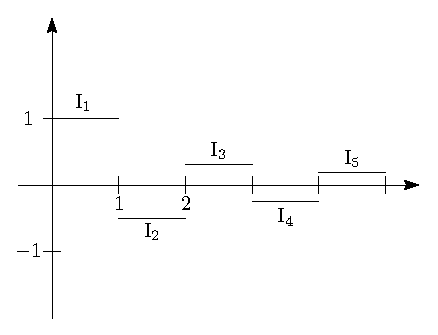
\includegraphics[width=0.35\textwidth]{MA4L9_1.eps}
	\caption{Функция $f(x)$.}
	\label{9_1}
\end{figure}
$$
	\lim\limits_{c \to \infty}\ddint{0}{c}f(x)dx = \ddsum{n = 1}{\infty}\dfrac{(-1)^{n-1}}{n} = \ln{2}, \quad N-1 < c < N \Rightarrow \left|\ddint{0}{c}f(x)dx - \ddsum{n = 1}{N}\dfrac{(-1)^{n-1}}{n}\right|\leq \dfrac{2}{N-1} \to 0
$$
Возникает вопрос, а с точки зрения нового определения будет эта функция интегрируема или нет? Если допускать исчерпание, как в многомерном случае, то можно выбрать любую перестановку отрезков: $\MI_{\varphi(1)}, \MI_{\varphi(2)}, \dotsc$ и брать объединение:
$$
	E_m = \bigcup\limits_{k = 1}^{m}\MI_{\varphi(k)} \Rightarrow \ddint{E_m}{}f(x)dx \xrightarrow[m \to \infty]{} \text{перестановка ряда } \ddsum{n = 1}{\infty}\dfrac{(-1)^{n-1}}{n} = A
$$
А мы знаем, что перестановкой такого ряда можно получить произвольное число $A$ или $\pm \infty$ (теорема Римана). По итогу окажется (без доказательства), что никакой условной сходимости в новом определении не будет.

\begin{prop}
	Пусть $E$ - допустимое множество, $f$ - интегрируема по Риману на $E$ (в обычном смысле). Если $\{E_n\}$ это исчерпание $E$ (будут лежать в $\ME_f$, так как $E_n$ - это допустимые множества, а $f$ интегрируема на допустимом множестве $\Rightarrow$ интегрируема на подмножестве допустимого), то верно:
	\begin{enumerate}[label=\arabic*)]
		\item $|E| = \lim\limits_{m \to \infty}|E_m|$;
		\item $\int_{E}f(x)dx = \lim\limits_{m \to \infty}\int_{E_m}f(x)dx$;
	\end{enumerate}
\end{prop}
\begin{proof}\hfill
	\begin{enumerate}[label=\arabic*)]
		\item По определению: $E_m \subset E_{m+1} \subset E$, тогда: $|E_m| \uparrow$ (не возрастает) и $|E_m|\leq |E|$. Следовательно:
		$$
			\exists \, \lim\limits_{m \to \infty}|E_m| \wedge  \lim\limits_{m \to \infty}|E_m|\leq |E|
		$$
		Поскольку множества допустимы, то $\partial E_m, \, \partial E$ - это множества меры нуль по Лебегу, кроме того граница это замкнутое множество, а поскольку $E$ само было ограниченным $\Rightarrow$ это компакт, тогда:
		$$
			\forall \VE > 0, \, \exists \, \Delta_m, \Delta \colon |\Delta_m| < \dfrac{\VE}{2^m}, \, |\Delta| < \VE, \, \partial E_m \subset \Delta_m, \, \partial E \subset \Delta
		$$
		где $\Delta_m, \, \Delta$ - конечные объединения открытых кубов (взяли кубы, поскольку компакт $\Rightarrow$ конечное покрытие, а конечное объединение допустимых множеств это допустимое множество $\Rightarrow$ можно написать их объем), которые покрывают границу. Также, мы воспользовались тем, что граница это множество меры нуль $\Rightarrow$ есть ограничения на объем $\Delta_m, \Delta$. Тогда рассмотрим множество: 
		$$
			\MU_m = E_m \cup \Delta_m \cup \Delta
		$$  
		это открытое множество, поскольку если точка лежит в $\Delta_m, \Delta$, то там открытые множества $\Rightarrow$ входит с окрестностью, если точка лежит в $E_m \Rightarrow$ она либо внутренняя, либо граничная $\Rightarrow$ если граничная, то она в дельтах, если внутренняя $\Rightarrow$ с окрестностью входит в $E_m$. Тогда:
		$$
			\bigcup\limits_m \MU_m \supset \ovl{E} = E \cup \partial E
		$$
		поскольку $E_m$ закрыло $E$, а $\Delta_m, \Delta$ закрыли $\partial E$. Замыкание это компакт $\Rightarrow$ есть конечное подпокрытие, тогда:
		$$
			\MU_1 \cup \dotsc \cup \MU_N \supset E, \, E_m \subset E_{m+1} \Rightarrow \Delta \cup \Delta_1 \cup \dotsc \cup \Delta_N \cup E_N \supset E \Rightarrow 
		$$
		$$
			\Rightarrow |E| \leq |E_N| + |\Delta_1| + \dotsc + |\Delta_N| + |\Delta| \leq |E_N| + 2 \VE
		$$
		Поскольку $N$ - произвольное, то:
		$$
			|E| \leq \lim\limits_{N \to \infty}|E_N| + 2\VE \xrightarrow[\VE \to 0]{} \lim\limits_{N \to \infty}|E_N|
		$$
		Заметим, что все это можно было не делать, если бы воспользовались теоремой Лебега (см. далее в курсе). Возьмем $\chi_{E_m}(x)$ и $\chi_E(x)$, $E_m \subset E_{m+1}$ и $\cup_m E_m = E \subset \MI$, где $\MI$ - некоторый брус, тогда:
		$$
			|E_m| = \ddint{\MI}{}\chi_{E_m}(x)dx, \, |E| = \ddint{\MI}{}\chi_E(x)dx
		$$
		$$
			0 \leq \chi_{E_m}(x) \leq 1 \wedge \forall x \in \MI, \, \chi_{E_m}(x) \to \chi_{E}(x)
		$$
		функции индикаторы - ограничены и последнее верно в силу того, что если точка не лежит в $E$, то она не лежит ни в каком $E_m$ и там, и там нули, если лежит в $E$, то верно: 
		$$
			\exists \, k \colon x \in E_k \Rightarrow \forall m > k, \, x \in E_m
		$$
		Теорема Лебега о мажорируемой сходимости даёт нам $|E_m| \to |E|$;
		\item Следует из предыдущего пункта:
		$$
			\left| \ddint{E}{}f(x)dx - \ddint{E_m}{}f(x)dx \right| = \left|\ddint{E\setminus E_m}{}f(x)dx \right| \leq \sup\limits_{E}|f(x)|{\cdot}(|E| - |E_m|) \xrightarrow[m\to \infty]{} 0
		$$
	\end{enumerate}
\end{proof}
Таким образом, в случае допустимого $E$ мы понимаем, как нам считать интегралы. В случая, когда $E$ не является допустимым, то хотелось бы понять как оно будет работать, поскольку на каждое исчерпание делать своё исследование - совсем не целесообразно.

\begin{theorem}
	Пусть $f \geq 0$ и $\ME_f \neq \VN$, тогда из существования предела: $\lim\limits_{m \to \infty}\int_{E_m}f(x)dx$ для одного исчерпания $\{E_m\} \in \ME_f$ следует существование предела для всякого исчерпания и эти пределы равны.
\end{theorem}
\begin{proof}
	Пусть $\{E_m\}$ - исчерпание по которому $\exists \, \lim\limits_{m \to \infty}\int_{E_m}f(x)dx$, возьмем другое исчерпание $\{D_k\}$ из $\ME_f$. Заметим, что если взять множества $\{E_m \cap D_k\}_m$, то это будет исчерпанием $D_k$:
	$$
		D_k \subset E, \, \bigcup\limits_m E_m = E \Rightarrow \bigcup\limits_{m}(E_m \cap D_k) = D_k
	$$
	По доказанному утверждению будет верно:
	$$
		\ddint{D_k}{}f(x)dx = \lim\limits_{m \to \infty}\ddint{E_m \cap D_k}{}f(x)dx \leq \lim\limits_{m \to \infty}\ddint{E_m }{}f(x)dx
	$$
	где последнее верно в силу того, что $f(x) \geq 0$ и увеличелась область интегрирования $\Rightarrow$ интеграл мог лишь увеличиться: 
	$$
		E_m = (E_m \cap D_k) \cup (E_m \setminus D_k), \, (E_m \cap D_k) \cap (E_m \setminus D_k) = \VN \Rightarrow 
	$$
	$$
		\Rightarrow \ddint{E_m}{}f(x)dx =  \ddint{E_m \cap D_k}{}f(x)dx + \ddint{E_m \setminus D_k}{}f(x)dx \geq \ddint{E_m \cap D_k}{}f(x)dx + 0 = \ddint{E_m \cap D_k}{}f(x)dx
	$$
	Также заметим, что: 
	$$
		D_k \subset D_{k +1 } \wedge f(x) \geq 0 \Rightarrow \ddint{D_k}{}f(x)dx \leq \ddint{D_{k+1}}{}f(x)dx \leq \lim\limits_{m \to \infty}\ddint{E_m }{}f(x)dx
	$$ 
	то есть последовательность интегралов не возрастает и ограничена, следовательно:
	$$
		\exists \, \lim \limits_{k \to \infty} \ddint{D_k}{}f(x)dx \leq  \lim\limits_{m \to \infty}\ddint{E_m }{}f(x)dx
	$$
	Меняем местами эти исчерпания и получаем равенство.
\end{proof}
\begin{corollary}
	Пусть $\VN \neq \ME_f \subset \ME_g$ и $|f| \leq g$, тогда из интегрируемости $g$ по множеству $E$ следует интегрируемость $f$ по множеству $E$.
\end{corollary}
\begin{proof}
	Рассмотрим функции: 
	$$
		f^+(x) = \max\{f(x), 0\} \geq 0, \, f^{-}(x) = \max\{-f(x),0\} \geq 0
	$$
	Тогда: $f(x) = f^+(x) - f^-(x)$, кроме того, мы подставили функцию $f(x)$ в $\max\{x,0\}, \, \max\{-x,0\}$ - Липшицевы функции (хотя нам достаточно просто непрерывности функции $\Rightarrow$ получаем подстановку интегрируемой функции в непрерывную, см. следствие $2$ лекции $4$) $\Rightarrow f^+(x), f^-(x)$ интегрируемы там же, где и $f(x)$, тогда: 
	$$
		\ME_f \subset \ME_{f^+}, \, \ME_f \subset \ME_{f^-}
	$$ 
	Заметим, что исчерпания для $f^+(x)$ и $f^-(x)$ могут иметь гораздо больше возможностей, чем просто $f$, например, если $f^-(x) \equiv 0$. Возьмем исчерпание $\{E_m\} \in \ME_f$, тогда:
	$$
		f^+(x) \leq |f(x)|\leq g(x) \Rightarrow \ddint{E_m}{}f^+(x)dx \leq \ddint{E_m}{}g(x)dx
	$$
	$$
		 f^-(x) \leq |f(x)|\leq g(x) \Rightarrow \ddint{E_m}{}f^-(x)dx \leq \ddint{E_m}{}g(x)dx
	$$
	По условию $\exists\, \lim\limits_{m \to \infty}\int_{E_m}g(x)dx \Rightarrow$ ограничены $\Rightarrow$ последовательность $\int_{E_m}f^+(x)dx$ - ограниченна и $\uparrow$ (не убывает) $\Rightarrow$ есть предел: $\exists \, \lim\limits_{m \to \infty}\int_{E_m}f^+(x)dx$, аналогично для $f^{-}(x) \colon \exists \, \lim\limits_{m \to \infty}\int_{E_m}f^-(x)dx$. Тогда по арифметике пределов и линейности обычного интеграла существует предел:
	$$
		\exists \, \lim\limits_{m \to \infty}\ddint{E_m}{}f(x)dx = \lim\limits_{m \to \infty}\ddint{E_m}{}(f^+(x) - f^-(x))dx = \lim\limits_{m \to \infty}\ddint{E_m}{}f^+(x)dx - \lim\limits_{m \to \infty}\ddint{E_m}{}f^-(x)dx
	$$
	Из существования пределов: $\exists \, \lim\limits_{m \to \infty}\int_{E_m}f^+(x)dx, \, \lim\limits_{m \to \infty}\int_{E_m}f^-(x)dx$ и теоремы доказанной выше следует, что $f^+(x)$ и $f^-(x)$ интегрируемы на $E$ в несобственном смысле. Тогда:
	$$
		\lim\limits_{m \to \infty}\ddint{E_m}{}f(x)dx = \lim\limits_{m \to \infty}\ddint{E_m}{}f^+(x)dx - \lim\limits_{m \to \infty}\ddint{E_m}{}f^-(x)dx = \ddint{E}{}f^+(x)dx - \ddint{E}{}f^-(x)dx 
	$$
	Следовательно, предел слева не зависит от $\{E_m\} \Rightarrow f(x)$ - интегрируема.
\end{proof}

\begin{rem}
	Пусть $\ME_f = \ME_{|f|} \neq \VN$, тогда $f$ интегрируема на $E$ в несобственном смысле $\Leftrightarrow |f|$ интегрируема на $E$ в несобственном смысле (без доказательства, его можно посмотреть в Зориче во $2$-м томе разложено в задачах). Следовательно, никакой условной сходимости нет.
\end{rem}

\textbf{Пример}: Рассмотрим следующий несобственный интеграл ($\MR^2$ не является допустимым множеством):
$$
	\iint\limits_{\MR^2}e^{-x^2 - y^2}dxdy
$$
Хотим понять, сходится ли этот интеграл. Попробуем посмотреть на исчерпание квадратами:
$$
	\iint\limits_{\MR^2}e^{-x^2 - y^2}dxdy = \lim\limits_{m \to \infty}\iint\limits_{[-m,m]\times[-m,m]}e^{-x^2 - y^2}dxdy = \lim\limits_{m \to \infty}\ddint{-m}{m}\left(\ddint{-m}{m}e^{-x^2}{\cdot}e^{-y^2}dx\right)dy = (*)
$$
где в предпоследнем равенстве мы воспользовались теоремой Фубини. Мы знаем, что в одномерном случае интеграл  от $e^{-x^2}$ сходится на $\MR$, тогда:
$$
	(*) = \lim\limits_{m \to \infty}\ddint{-m}{m}e^{-x^2}dx{\cdot}\ddint{-m}{m}e^{-y^2}dy = \left(\ddint{-\infty}{\infty}e^{-t^2}dt\right)^2
$$
Возьмем другое исчерпание - шарами: $E_m = \{x \colon \|x\| < m\} \Rightarrow $ интеграл от этой функции по шару лучше всего считать в полярной системе координат, где:	
$$
	x = r\cos{\varphi}, \, y = r\sin{\varphi} \Rightarrow \MJ(r,\varphi) = 
	\begin{pmatrix}
		\cos{\varphi} & -r \sin{\varphi}\\
		\sin{\varphi} & r\cos{\varphi}
	\end{pmatrix} \Rightarrow |\MJ(r,\varphi)| = r
$$
и якобиан замены здесь $r \Rightarrow$ видно, что теорема о замене переменных здесь уже не работает, поскольку такая замена - не диффеоморфизм (поскольку у нас есть зануление якобиана в точке $0$ и нет однозначности, если $\varphi$ идет по полному обороту). Следовательно, отойдем от $0$ на какое-либо положительное $\delta > 0$ и сделаем вырезку полосы ширины $\delta$:
\begin{figure}[H]
	\centering
	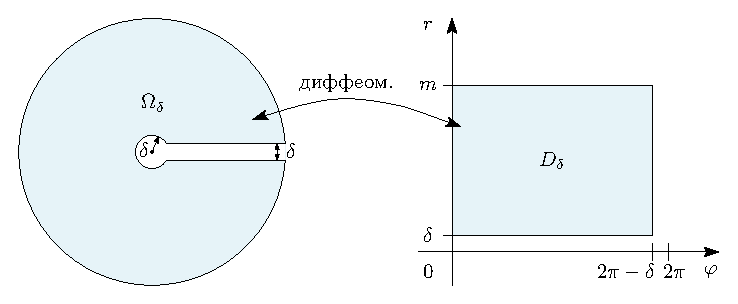
\includegraphics[width=0.75\textwidth]{MA4L9_2.eps}
	\caption{Диффеоморфизм для формулы замены переменной между $\Omega_\delta$ и $D_\delta$.}
	\label{9_2}
\end{figure}
Таким образом, получим диффеоморфизм между сферой с вырезкой и $[\delta,m] \times [0,2 \pi - \delta] \Rightarrow$ можем воспользоваться заменой координат, а затем можно устремить $\delta \to 0$ и проверить, что у интегралов справа и слева ничего не происходит при таком предельном переходе. Используя ФЗП:
$$
	\ddint{\Omega_\delta}{}e^{-x^2 - y^2}dxdy = \ddint{D_\delta}{}e^{-r^2}rdrd\varphi 
$$
Далее мы хотим $\delta \to 0$, возникает вопрос, почему мы придем к интегралу по $\Omega$ и интегралу по $D$ (если выражения под интегралами выше интегрируемы по $\Omega$ и по $D$)? По теореме $1$. Сделаем замену переменных:
$$
	\iint\limits_{E_m}{}e^{-x^2 - y^2}dxdy = \ddint{0}{2\pi}d\varphi \ddint{0}{m}e^{-r^2}rdr = 2\pi\ddint{0}{m}e^{-r^2}rdr = \pi\ddint{0}{m^2}e^{-t}dt = \pi(1 - e^{-m^2}) \xrightarrow[m \to \infty]{} \pi
$$
Поскольку под интегралом неотрицательная функция, то мы доказали, что этот интеграл сходится и равен $\pi \Rightarrow$ по теореме значение интеграла не зависит от выбора исчерпания, тогда:
$$
	\iint\limits_{\MR^2}e^{-x^2 - y^2}dxdy = \lim\limits_{m \to \infty}\iint\limits_{x^2 + y^2 \leq m}e^{-x^2 - y^2}dxdy = \pi
$$
$$
	\iint\limits_{\MR^2}e^{-x^2 - y^2}dxdy = \left(\ddint{-\infty}{\infty}e^{-t^2}dt\right)^2 = \pi \Rightarrow \ddint{-\infty}{\infty}e^{-t^2}dt = \sqrt{\pi}
$$
И мы снова получили значение интеграла Эйлера-Пуассона.
\begin{rem}
	Подобным же образом можно избавляться от особых точек: если в области есть плохие точки и мы можем вырезать - сделать замену - перейти обратно к пределу $\Rightarrow$ считается, что вы можете делать замены переменных. В частности, если такая точка одна и интегралы в ФЗП справа/слева существуют, то их результаты будут совпадать.
\end{rem}
\begin{rem}
	Отметим, что ФЗП для областей с особенностями разбирается во $2$-ом томе Зорича (замена переменных в кратных интегралах, теорема $2$).
\end{rem}

\textbf{Пример}: Рассмотрим множество $E = \{x \colon 0 < \|x\| < 1\}$ и функцию $f(x) = \tfrac{1}{\|x\|^p}$. Хотим выяснить при каких $p$ функция $f(x)$ интегрируема по множеству $E$? Рассмотрим интеграл по исчерпанию:
$$
	\ddint{\tfrac{1}{m} < \|x\| < 1}{}\dfrac{1}{\|x\|^p}dx = |x = \psi(\varphi_1,\dotsc,\varphi_{n-1}, r), \, \MJ = r^{n-1}{\cdot}g(\varphi_1,\dotsc,\varphi_{n-1})| =  
$$
$$
	= \ddint{\varphi_1, \dotsc, \varphi_{n-1}}{}d\varphi_1\dotsc d\varphi_{n-1}\ddint{\tfrac{1}{m}}{1}\dfrac{1}{r^p}{\cdot}r^{n-1}{\cdot}|g(\varphi)|dr = \ddint{\varphi_1, \dotsc, \varphi_{n-1}}{}|g(\varphi)|d\varphi_1\dotsc d\varphi_{n-1}\ddint{\tfrac{1}{m}}{1}\dfrac{1}{r^{p - n + 1}}dr
$$
где мы воспользовались заменой переменных и нам в этой ситуации не важно, как устроена функция от углов: $g(\varphi_1,\dotsc,\varphi_{n-1})$. Интеграл от $\varphi$ это некоторое ненулевое число, поскольку это интеграл от положительной функции $\Rightarrow$ нулём оказаться не может $\Rightarrow$ нас будет интересовать только интеграл справа: когда у него есть предел при $m \to \infty$? Это вопрос про то, когда сходится этот интеграл в нуле. Тогда:
$$
	\text{сходимость } \ddint{0}{1}\dfrac{1}{\|x\|^p}dx \Leftrightarrow \text{сходимость } \ddint{0}{1}\dfrac{1}{r^{p - n + 1}}dr
$$
То есть, сходимость есть при: $p - n + 1 < 1 \Leftrightarrow p < n$. Это происходит из-за того, что появляется якобиан и помогает интегрируемости. Попробуем всё же осознать чему равен интеграл от углов, для этого возьмем интеграл от $1$ по единичному шару $\omega_n$ и перейдем в полярную систему координат:
$$
	|\omega_n| = \ddint{\|x\| < 1}{}1dx = \ddint{\varphi_1,\dotsc, \varphi_{n-1}}{}|g(\varphi)|d\varphi\ddint{0}{1}r^{n-1}dr = \dfrac{1}{n}\ddint{\varphi_1,\dotsc, \varphi_{n-1}}{}|g(\varphi)|d\varphi \Rightarrow \ddint{\varphi_1,\dotsc, \varphi_{n-1}}{}|g(\varphi)|d\varphi = n{\cdot}|\omega_n|
$$
Заодно мы умеем переходить в полярную систему координат, когда под интегралом стоит радиальная функция и это на самом деле почти все типичные ситуации, когда это надо уметь делать:
$$
	\ddint{\|x\| < R}{} f(\|x\|)dx = n{\cdot}|\omega_n|{\cdot}\ddint{0}{R}f(r){\cdot}r^{n-1}dr
$$


\end{document}